% Root file used ashow macros
\documentclass{beamer}
\usepackage{tikz}
\usetikzlibrary{calc,arrows.meta,patterns}
\usepackage{xcolor}
\usepackage{multicol}
\usepackage{amsmath}

% ================================================================
% Answer-overlay helpers
% ================================================================
\newcommand{\ablank}[1]{%
  \alt<2>{\textcolor{red}{#1}}{\underline{\phantom{#1}}}%
}
\newcommand{\ashow}[1]{\uncover<2->{\textcolor{red}{\small #1}}}
\newcommand{\ashowq}[1]{\alt<2->{\textcolor{red}{\small #1}}{?}}

% Answers drawn straight on to a TikZ diagram, revealed on overlay 2 like \ashow.
% Space is reserved on overlay 1, so the diagram does not move between slides.
\usetikzlibrary{overlay-beamer-styles}
\tikzset{
  ans/.style     = {red, thick, visible on=<2->},
  ansfill/.style = {red!15, visible on=<2->},
  anslab/.style  = {red, font=\tiny, visible on=<2->},
}

\title{Averages: Mean \& Median}
\author{}
\date{}

% Lego tower: \legotower{x-offset}{height}{colour}
% Each brick is 0.65 wide x 0.55 tall, with two studs
\newcommand{\legotower}[3]{%
  \foreach \i in {1,...,#2}{%
    \draw[fill=#3!55, draw=#3!80!black, line width=0.35pt]
      (#1, {(\i-1)*0.55}) rectangle (#1+0.65, {\i*0.55});
    \draw[fill=#3!80, draw=#3!80!black, line width=0.2pt]
      (#1+0.15,{(\i-1)*0.55+0.38}) circle (0.08);
    \draw[fill=#3!80, draw=#3!80!black, line width=0.2pt]
      (#1+0.44,{(\i-1)*0.55+0.38}) circle (0.08);
  }%
}

  \newcommand{\lego}[3]{%
    \foreach \ii in {1,...,#2}{%
      \draw[fill=#3!55,draw=#3!80!black,line width=0.3pt]
        (#1,{(\ii-1)*0.42}) rectangle (#1+0.6,{\ii*0.42});
      \draw[fill=#3!80,draw=#3!80!black,line width=0.15pt]
        (#1+0.13,{(\ii-1)*0.42+0.30}) circle (0.07);
      \draw[fill=#3!80,draw=#3!80!black,line width=0.15pt]
        (#1+0.40,{(\ii-1)*0.42+0.30}) circle (0.07);
    }%
  }


  \newcommand{\legob}[3]{%
    \foreach \ii in {1,...,#2}{%
      \draw[fill=#3!55,draw=#3!80!black,line width=0.3pt]
        (#1,{(\ii-1)*0.42}) rectangle (#1+0.6,{\ii*0.42});
      \draw[fill=#3!80,draw=#3!80!black,line width=0.15pt]
        (#1+0.13,{(\ii-1)*0.42+0.30}) circle (0.07);
      \draw[fill=#3!80,draw=#3!80!black,line width=0.15pt]
        (#1+0.40,{(\ii-1)*0.42+0.30}) circle (0.07);
    }%
  }

\begin{document}

\frame{\titlepage}

\begin{frame}{Contents}
\small
\begin{columns}[T]
\column{0.5\textwidth}
\textbf{Questions and short answers}
\begin{itemize}
  \item \hyperlink{q-st1}{\beamergotobutton{Starter 1}}
  \item \hyperlink{q-st2}{\beamergotobutton{Starter 2}}
  \item \hyperlink{q-st3}{\beamergotobutton{Starter 3}}
  \item \hyperlink{q-st4}{\beamergotobutton{Starter 4}}
  \item \hyperlink{q-st5}{\beamergotobutton{Starter 5}}
\end{itemize}

\column{0.5\textwidth}
\textbf{Worked solutions}
\begin{itemize}
  \item \hyperlink{work-st1}{\beamergotobutton{Starter 1}}
  \item \hyperlink{work-st2}{\beamergotobutton{Starter 2}}
  \item \hyperlink{work-st3}{\beamergotobutton{Starter 3}}
  \item \hyperlink{work-st4}{\beamergotobutton{Starter 4}}
  \item \hyperlink{work-st5}{\beamergotobutton{Starter 5}}
\end{itemize}
\end{columns}
\end{frame}

%------------------------------------------------
% STARTER 1
%------------------------------------------------
\begin{frame}{Starter 1}
\hypertarget{q-st1}{}
\vspace{-0.8em}
\begin{columns}[T]

\column{0.33\textwidth}
\begin{center}

% Diagram 1: towers 1,3,2  (scale 0.9, bricks 0.5 tall)
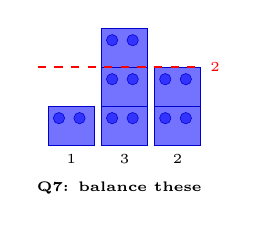
\begin{tikzpicture}[scale=0.9]
  \legotower{0.00}{1}{blue}
  \legotower{0.75}{3}{blue}
  \legotower{1.50}{2}{blue}
  \node[below,font=\tiny] at (0.325,0) {1};
  \node[below,font=\tiny] at (1.075,0) {3};
  \node[below,font=\tiny] at (1.825,0) {2};
  \node[below,font=\tiny\bfseries] at (1.0,{-0.38})
    {\textbf{Q7}: balance these};
  \draw[ans, dashed] (-0.15,1.1) -- (2.15,1.1);
  \node[anslab, right] at (2.15,1.1) {2};
\end{tikzpicture}

\vspace{0.55em}

% Diagram 2: towers 1,3,5,3,3  (scale 0.78 to fit width)
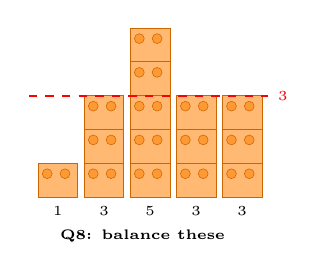
\begin{tikzpicture}[scale=0.78]
  \legotower{0.00}{1}{orange}
  \legotower{0.75}{3}{orange}
  \legotower{1.50}{5}{orange}
  \legotower{2.25}{3}{orange}
  \legotower{3.00}{3}{orange}
  \node[below,font=\tiny] at (0.325,0) {1};
  \node[below,font=\tiny] at (1.075,0) {3};
  \node[below,font=\tiny] at (1.825,0) {5};
  \node[below,font=\tiny] at (2.575,0) {3};
  \node[below,font=\tiny] at (3.325,0) {3};
  \node[below,font=\tiny\bfseries] at (1.7,{-0.38})
    {\textbf{Q8}: balance these};
  \draw[ans, dashed] (-0.15,1.65) -- (3.75,1.65);
  \node[anslab, right] at (3.75,1.65) {3};
\end{tikzpicture}

\end{center}

\column{0.67\textwidth}
\footnotesize
\vspace{0.2em}
\begin{enumerate}\itemsep1pt
  \begin{multicols}{2}
    \item $12 \div 4 = \ashowq{3}$
    \item $18 \div 3 = \ashowq{6}$
  \end{multicols}
  \begin{multicols}{2}
    \item $15 \div 3 = \ashowq{5}$
    \item $28 \div 4 = \ashowq{7}$
  \end{multicols}
  \item Four friends share 20 sweets equally. How many do they each get? \ashow{5 sweets}
  \item Three children have 2, 5 and 8 stickers. They combine them and share them equally. How many does each child get? \ashow{5 stickers}
  \item Draw a picture of the top towers (left), balanced to the same height without changing the total number of bricks.
  \item Draw a picture of the bottom towers (left), balanced to the same height without changing the total number of bricks.
\end{enumerate}

\end{columns}
\end{frame}

\begin{frame}{Worked Solution: Starter 1, Question 1}
\hypertarget{work-st1}{}
\textbf{Question:} \(12 \div 4 = ?\)

\textbf{Worked Solution:}
Since \(4 \times 3 = 12\),
\[
12 \div 4 = 3.
\]
\end{frame}

\begin{frame}{Worked Solution: Starter 1, Question 2}
\textbf{Question:} \(18 \div 3 = ?\)

\textbf{Worked Solution:}
Since \(3 \times 6 = 18\),
\[
18 \div 3 = 6.
\]
\end{frame}

\begin{frame}{Worked Solution: Starter 1, Question 3}
\textbf{Question:} \(15 \div 3 = ?\)

\textbf{Worked Solution:}
Since \(3 \times 5 = 15\),
\[
15 \div 3 = 5.
\]
\end{frame}

\begin{frame}{Worked Solution: Starter 1, Question 4}
\textbf{Question:} \(28 \div 4 = ?\)

\textbf{Worked Solution:}
Since \(4 \times 7 = 28\),
\[
28 \div 4 = 7.
\]
\end{frame}

\begin{frame}{Worked Solution: Starter 1, Question 5}
\textbf{Question:} Four friends share 20 sweets equally. How many do they each get?

\textbf{Worked Solution:}
Sharing equally means dividing the total by the number of friends:
\[
20 \div 4 = 5.
\]
Each friend gets \(5\) sweets.
\end{frame}

\begin{frame}{Worked Solution: Starter 1, Question 6}
\textbf{Question:} Three children have 2, 5 and 8 stickers. They combine them and share them equally. How many does each child get?

\textbf{Worked Solution:}
Total stickers:
\[
2 + 5 + 8 = 15.
\]
There are 3 children, so each child gets
\[
15 \div 3 = 5
\]
stickers.
\end{frame}

\begin{frame}{Worked Solution: Starter 1, Question 7}
\textbf{Question:} Draw a picture of the top towers, balanced to the same height without changing the total number of bricks.

\textbf{Worked Solution:}
The top towers have heights \(1, 3, 2\).

Total bricks:
\[
1 + 3 + 2 = 6.
\]
There are 3 towers, so the balanced height is
\[
6 \div 3 = 2.
\]
The picture should show all the bricks levelled out at height \(2\).
\end{frame}

\begin{frame}{Worked Solution: Starter 1, Question 8}
\textbf{Question:} Draw a picture of the bottom towers, balanced to the same height without changing the total number of bricks.

\textbf{Worked Solution:}
The bottom towers have heights \(1, 3, 5, 3, 3\).

Total bricks:
\[
1 + 3 + 5 + 3 + 3 = 15.
\]
There are 5 towers, so the balanced height is
\[
15 \div 5 = 3.
\]
The picture should show all the bricks levelled out at height \(3\).
\end{frame}

%------------------------------------------------
% STARTER 2
%------------------------------------------------
\begin{frame}{Starter 2}
\hypertarget{q-st2}{}
\vspace{-0.8em}
\begin{columns}[T]

\column{0.33\textwidth}
\begin{center}

% Diagram 1: towers 3,5,4,8 — brick height 0.42 to keep 8-tower in frame
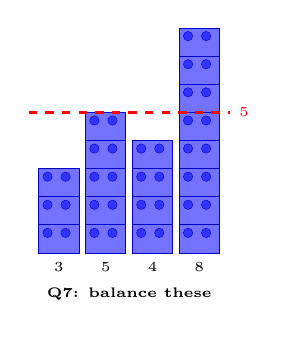
\begin{tikzpicture}[scale=0.85]

  \lego{0.00}{3}{blue}
  \lego{0.70}{5}{blue}
  \lego{1.40}{4}{blue}
  \lego{2.10}{8}{blue}
  \node[below,font=\tiny] at (0.30,0) {3};
  \node[below,font=\tiny] at (1.00,0) {5};
  \node[below,font=\tiny] at (1.70,0) {4};
  \node[below,font=\tiny] at (2.40,0) {8};
  \node[below,font=\tiny\bfseries] at (1.35,{-0.38})
    {\textbf{Q7}: balance these};
  \draw[ans, dashed] (-0.15,2.10) -- (2.85,2.10);
  \node[anslab, right] at (2.85,2.10) {5};
\end{tikzpicture}

\vspace{0.45em}

% Diagram 2: towers 1,5,2,8,4
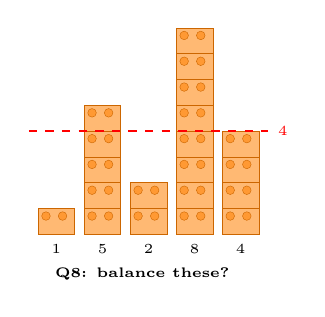
\begin{tikzpicture}[scale=0.78]

  \legob{0.00}{1}{orange}
  \legob{0.75}{5}{orange}
  \legob{1.50}{2}{orange}
  \legob{2.25}{8}{orange}
  \legob{3.00}{4}{orange}
  \node[below,font=\tiny] at (0.30,0) {1};
  \node[below,font=\tiny] at (1.05,0) {5};
  \node[below,font=\tiny] at (1.80,0) {2};
  \node[below,font=\tiny] at (2.55,0) {8};
  \node[below,font=\tiny] at (3.30,0) {4};
  \node[below,font=\tiny\bfseries] at (1.7,{-0.38})
    {\textbf{Q8}: balance these?};
  \draw[ans, dashed] (-0.15,1.68) -- (3.75,1.68);
  \node[anslab, right] at (3.75,1.68) {4};
\end{tikzpicture}

\end{center}

\column{0.67\textwidth}
\footnotesize
\vspace{0.2em}
  \begin{multicols}{2}
  \begin{enumerate}
    \item $7 \times 8 = \ashowq{56}$
    \item $63 \div 7 = \ashowq{9}$
    \end{enumerate}
  \end{multicols}
  \begin{multicols}{2}
  \begin{enumerate}
  \setcounter{enumi}{2}
    \item $48 \div 8 = \ashowq{6}$
    \item $5 \times 9 = \ashowq{45}$
    \end{enumerate}
  \end{multicols}
  \begin{enumerate}
  \setcounter{enumi}{4}
  \item Five children have 4, 7, 3, 6, 5 marbles. Shared equally, how many each? \ashow{5 marbles}
  \item Six friends earn £8, £14, £10, £6, £12, £10 at a car wash. Split fairly — how much each? \ashow{\pounds10 each}
  \item Eight runners finish in 54, 48, 61, 57, 50, 63, 55, 52 s. Without doing any calculations, estimate the average time. \ashow{about 55 s}
  \item What heights would the top towers balance out to? \ashow{5 bricks high}
  \item What heights would the bottom towers balance out to? \ashow{4 bricks high}
\end{enumerate}

\end{columns}
\end{frame}

\begin{frame}{Worked Solution: Starter 2, Question 1}
\hypertarget{work-st2}{}
\textbf{Question:} \(7 \times 8 = ?\)

\textbf{Worked Solution:}
\[
7 \times 8 = 56.
\]
This is one of the times-table facts for \(7\) and \(8\).
\end{frame}

\begin{frame}{Worked Solution: Starter 2, Question 2}
\textbf{Question:} \(63 \div 7 = ?\)

\textbf{Worked Solution:}
Since \(7 \times 9 = 63\),
\[
63 \div 7 = 9.
\]
\end{frame}

\begin{frame}{Worked Solution: Starter 2, Question 3}
\textbf{Question:} \(48 \div 8 = ?\)

\textbf{Worked Solution:}
Since \(8 \times 6 = 48\),
\[
48 \div 8 = 6.
\]
\end{frame}

\begin{frame}{Worked Solution: Starter 2, Question 4}
\textbf{Question:} \(5 \times 9 = ?\)

\textbf{Worked Solution:}
\[
5 \times 9 = 45,
\]
because \(9 \times 5 = 45\).
\end{frame}

\begin{frame}{Worked Solution: Starter 2, Question 5}
\textbf{Question:} Five children have 4, 7, 3, 6, 5 marbles. Shared equally, how many each?

\textbf{Worked Solution:}
Total marbles:
\[
4 + 7 + 3 + 6 + 5 = 25.
\]
There are 5 children, so each child gets
\[
25 \div 5 = 5
\]
marbles.
\end{frame}

\begin{frame}{Worked Solution: Starter 2, Question 6}
\textbf{Question:} Six friends earn \pounds8, \pounds14, \pounds10, \pounds6, \pounds12, \pounds10 at a car wash. Split fairly — how much each?

\textbf{Worked Solution:}
Total earned:
\[
8 + 14 + 10 + 6 + 12 + 10 = 60
\]
pounds.
There are 6 friends, so each gets
\[
60 \div 6 = 10
\]
pounds, i.e. \(\pounds10\) each.
\end{frame}

\begin{frame}{Worked Solution: Starter 2, Question 7}
\textbf{Question:} Eight runners finish in 54, 48, 61, 57, 50, 63, 55, 52 s. Without doing any calculations, estimate the average time.

\textbf{Worked Solution:}
The times are spread fairly evenly around \(55\) s: some are a little above and some are a little below. So a good estimate is
\[
\text{about } 55 \text{ seconds}.
\]
Checking exactly:
\[
54+48+61+57+50+63+55+52=440,
\]
so the mean is
\[
440 \div 8 = 55 \text{ s}.
\]
The estimate is exact.
\end{frame}

\begin{frame}{Worked Solution: Starter 2, Question 8}
\textbf{Question:} What heights would the top towers balance out to?

\textbf{Worked Solution:}
The top towers have heights \(3, 5, 4, 8\).

Total bricks:
\[
3 + 5 + 4 + 8 = 20.
\]
There are 4 towers, so the balanced height is
\[
20 \div 4 = 5
\]
bricks high.
\end{frame}

\begin{frame}{Worked Solution: Starter 2, Question 9}
\textbf{Question:} What heights would the bottom towers balance out to?

\textbf{Worked Solution:}
The bottom towers have heights \(1, 5, 2, 8, 4\).

Total bricks:
\[
1 + 5 + 2 + 8 + 4 = 20.
\]
There are 5 towers, so the balanced height is
\[
20 \div 5 = 4
\]
bricks high.
\end{frame}

%------------------------------------------------
% STARTER 3
%------------------------------------------------
\begin{frame}{Starter 3}
\hypertarget{q-st3}{}
\vspace{-0.8em}

\footnotesize
\vspace{0.2em}
\begin{enumerate}\itemsep1pt
  \begin{multicols}{2}
    \item $3 + 4 + 7 = \ashowq{14}$
    \item $15+27+18=\ashowq{60}$
    \item $60\div 4=\ashowq{15}$
    \item $-15 \div 3=\ashowq{-5}$
  \end{multicols}
  \vspace{-1em}
  \item What is the mean of: $4,\ 6,\ 2,\ 8$ \ashow{5}
  \item What is the mean  of: $3,\ 9,\ 5,\ 7,\ 1$ \ashow{5}
  \item What is the mean  of: $-3,\ 5,\ -1,\ 7,\ 2$ \ashow{2}
  \item What is the mean  of: $-8,\ -2,\ -5,\ -1,\ -4$ \ashow{$-4$}
\end{enumerate}

\begin{enumerate}\itemsep1pt
  \setcounter{enumi}8
  \item The mean of four numbers is 9. Three are 6, 11 and 8. Find the fourth. \ashow{11}
  \item The mean of $3,\ 7,\ x,\ 10$ is $8$. What is $x$? \ashow{12}
\end{enumerate}


\end{frame}

\begin{frame}{Worked Solution: Starter 3, Question 1}
\hypertarget{work-st3}{}
\textbf{Question:} \(3 + 4 + 7 = ?\)

\textbf{Worked Solution:}
\[
3 + 4 + 7 = 14.
\]
Add in stages: \(3 + 4 = 7\), then \(7 + 7 = 14\).
\end{frame}

\begin{frame}{Worked Solution: Starter 3, Question 2}
\textbf{Question:} \(15 + 27 + 18 = ?\)

\textbf{Worked Solution:}
\[
15 + 27 + 18 = 60.
\]
For example, \(15 + 27 = 42\), and \(42 + 18 = 60\).
\end{frame}

\begin{frame}{Worked Solution: Starter 3, Question 3}
\textbf{Question:} \(60 \div 4 = ?\)

\textbf{Worked Solution:}
Since \(4 \times 15 = 60\),
\[
60 \div 4 = 15.
\]
\end{frame}

\begin{frame}{Worked Solution: Starter 3, Question 4}
\textbf{Question:} \(-15 \div 3 = ?\)

\textbf{Worked Solution:}
First \(15 \div 3 = 5\).
A negative number divided by a positive number is negative, so
\[
-15 \div 3 = -5.
\]
\end{frame}

\begin{frame}{Worked Solution: Starter 3, Question 5}
\textbf{Question:} What is the mean of \(4, 6, 2, 8\)?

\textbf{Worked Solution:}
Sum:
\[
4 + 6 + 2 + 8 = 20.
\]
There are 4 numbers, so
\[
\text{mean} = \frac{20}{4} = 5.
\]
\end{frame}

\begin{frame}{Worked Solution: Starter 3, Question 6}
\textbf{Question:} What is the mean of \(3, 9, 5, 7, 1\)?

\textbf{Worked Solution:}
Sum:
\[
3 + 9 + 5 + 7 + 1 = 25.
\]
There are 5 numbers, so
\[
\text{mean} = \frac{25}{5} = 5.
\]
\end{frame}

\begin{frame}{Worked Solution: Starter 3, Question 7}
\textbf{Question:} What is the mean of \(-3, 5, -1, 7, 2\)?

\textbf{Worked Solution:}
Sum the numbers:
\[
-3 + 5 - 1 + 7 + 2 = 10.
\]
There are 5 numbers, so
\[
\text{mean} = \frac{10}{5} = 2.
\]
\end{frame}

\begin{frame}{Worked Solution: Starter 3, Question 8}
\textbf{Question:} What is the mean of \(-8, -2, -5, -1, -4\)?

\textbf{Worked Solution:}
Sum the numbers:
\[
-8 - 2 - 5 - 1 - 4 = -20.
\]
There are 5 numbers, so
\[
\text{mean} = \frac{-20}{5} = -4.
\]
\end{frame}

\begin{frame}{Worked Solution: Starter 3, Question 9}
\textbf{Question:} The mean of four numbers is 9. Three are 6, 11 and 8. Find the fourth.

\textbf{Worked Solution:}
If the mean of 4 numbers is 9, their total is
\[
4 \times 9 = 36.
\]
The three known numbers add to
\[
6 + 11 + 8 = 25.
\]
So the fourth number is
\[
36 - 25 = 11.
\]
\end{frame}

\begin{frame}{Worked Solution: Starter 3, Question 10}
\textbf{Question:} The mean of \(3, 7, x, 10\) is \(8\). What is \(x\)?

\textbf{Worked Solution:}
If the mean of 4 numbers is 8, their total is
\[
4 \times 8 = 32.
\]
The known numbers add to
\[
3 + 7 + 10 = 20.
\]
Therefore
\[
x = 32 - 20 = 12.
\]
\end{frame}

%------------------------------------------------
% STARTER 4
%------------------------------------------------
\begin{frame}{Starter 4}
\hypertarget{q-st4}{}
\vspace{-0.8em}

\begin{columns}[T]

% ---------------- LEFT COLUMN ----------------
\column{0.33\textwidth}

\begin{center}

\vspace{7em}

% Dot plot: house prices with outlier
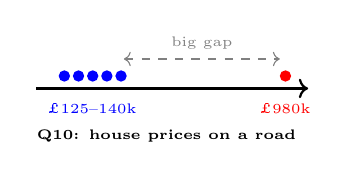
\begin{tikzpicture}[scale=0.72]

  \draw[thick,->] (-0.2,0) -- (4.6,0);

  \foreach \xd in {0.3,0.55,0.8,1.05,1.3}{
    \fill[blue] (\xd,0.22) circle (0.1);
  }

  \fill[red] (4.2,0.22) circle (0.1);

  \node[below,font=\tiny,blue] at (0.8,-0.1)
    {\pounds125--140k};

  \node[below,font=\tiny,red] at (4.2,-0.1)
    {\pounds980k};

  \draw[<->,dashed,gray]
    (1.35,0.52) -- (4.1,0.52)
    node[midway,above,font=\tiny,gray]{big gap};

  \node[below,font=\tiny\bfseries]
    at (2.1,-0.55)
    {\textbf{Q10}: house prices on a road};

\end{tikzpicture}

\end{center}

% ---------------- RIGHT COLUMN ----------------
\column{0.67\textwidth}

\footnotesize
\vspace{0.2em}

% First four quick questions
\begin{multicols}{2}
\begin{enumerate}\itemsep1pt
  \item $4+2+10=\ashowq{16}$
  \item $-4+9=\ashowq{5}$
  \item $-3-5=\ashowq{-8}$
  \item $6\times4=\ashowq{24}$
\end{enumerate}
\end{multicols}

% Remaining questions
\begin{enumerate}\itemsep1pt
\setcounter{enumi}{4}

  \item Order smallest to largest:
  $8,3,11,5,7$.
  Which is the middle value? \ashow{7}

  \item Order:
  $21,14,9,35,17,28,6$.
  Which is the middle value? \ashow{17}

  \item For $3,7,8,9,41$:
  \textit{estimate} whether the middle value is above or below the mean.
  Then check. \ashow{below: median $8$, mean $13.6$}

  \item What is the middle value of:
  $-7,\ -2,\ -5,\ 1,\ -1,\ 3,\ -3$ \ashow{$-2$}

  \item What is the middle value of:
  $\tfrac{1}{2},\ \tfrac{1}{4},\ \tfrac{3}{4},\ \tfrac{1}{8},\ \tfrac{5}{8}$ \ashow{$\frac{1}{2}$}

  \item House prices on a road are:
  \pounds130k,
  \pounds125k,
  \pounds140k,
  \pounds128k,
  \pounds135k,
  \textcolor{red}{\pounds980k}.

  Why might the mean not be helpful? \ashow{the \pounds980k outlier pulls the mean up}

\end{enumerate}

\end{columns}

\end{frame}

\begin{frame}{Worked Solution: Starter 4, Question 1}
\hypertarget{work-st4}{}
\textbf{Question:} \(4 + 2 + 10 = ?\)

\textbf{Worked Solution:}
\[
4 + 2 + 10 = 16.
\]
Add in stages: \(4 + 2 = 6\), then \(6 + 10 = 16\).
\end{frame}

\begin{frame}{Worked Solution: Starter 4, Question 2}
\textbf{Question:} \(-4 + 9 = ?\)

\textbf{Worked Solution:}
Starting at \(-4\) and moving up \(9\) gives
\[
-4 + 9 = 5.
\]
Equivalently, \(9 - 4 = 5\).
\end{frame}

\begin{frame}{Worked Solution: Starter 4, Question 3}
\textbf{Question:} \(-3 - 5 = ?\)

\textbf{Worked Solution:}
Subtracting \(5\) from \(-3\) means moving further down the number line:
\[
-3 - 5 = -8.
\]
\end{frame}

\begin{frame}{Worked Solution: Starter 4, Question 4}
\textbf{Question:} \(6 \times 4 = ?\)

\textbf{Worked Solution:}
\[
6 \times 4 = 24,
\]
because \(4 + 4 + 4 + 4 + 4 + 4 = 24\).
\end{frame}

\begin{frame}{Worked Solution: Starter 4, Question 5}
\textbf{Question:} Order \(8, 3, 11, 5, 7\) smallest to largest. Which is the middle value?

\textbf{Worked Solution:}
In order:
\[
3,\ 5,\ 7,\ 8,\ 11.
\]
There are 5 numbers, so the middle value is the 3rd number:
\[
7.
\]
\end{frame}

\begin{frame}{Worked Solution: Starter 4, Question 6}
\textbf{Question:} Order \(21, 14, 9, 35, 17, 28, 6\). Which is the middle value?

\textbf{Worked Solution:}
In order:
\[
6,\ 9,\ 14,\ 17,\ 21,\ 28,\ 35.
\]
There are 7 numbers, so the middle value is the 4th number:
\[
17.
\]
\end{frame}

\begin{frame}{Worked Solution: Starter 4, Question 7}
\textbf{Question:} For \(3, 7, 8, 9, 41\): estimate whether the middle value is above or below the mean. Then check.

\textbf{Worked Solution:}
The middle value, or median, is \(8\).

The mean is
\[
\frac{3 + 7 + 8 + 9 + 41}{5}
= \frac{68}{5}
= 13.6.
\]
So the middle value \(8\) is below the mean. The large value \(41\) pulls the mean upwards.
\end{frame}

\begin{frame}{Worked Solution: Starter 4, Question 8}
\textbf{Question:} What is the middle value of \(-7, -2, -5, 1, -1, 3, -3\)?

\textbf{Worked Solution:}
Write the numbers in order:
\[
-7,\ -5,\ -3,\ -2,\ -1,\ 1,\ 3.
\]
There are 7 numbers, so the middle value is the 4th number:
\[
-2.
\]
\end{frame}

\begin{frame}{Worked Solution: Starter 4, Question 9}
\textbf{Question:} What is the middle value of \(\frac{1}{2}, \frac{1}{4}, \frac{3}{4}, \frac{1}{8}, \frac{5}{8}\)?

\textbf{Worked Solution:}
Write each fraction in eighths:
\[
\frac{4}{8},\ \frac{2}{8},\ \frac{6}{8},\ \frac{1}{8},\ \frac{5}{8}.
\]
In order:
\[
\frac{1}{8},\ \frac{2}{8},\ \frac{4}{8},\ \frac{5}{8},\ \frac{6}{8}.
\]
The middle value is
\[
\frac{4}{8} = \frac{1}{2}.
\]
\end{frame}

\begin{frame}{Worked Solution: Starter 4, Question 10}
\textbf{Question:} House prices on a road are \pounds130k, \pounds125k, \pounds140k, \pounds128k, \pounds135k, \pounds980k. Why might the mean not be helpful?

\textbf{Worked Solution:}
In thousands of pounds, the prices are
\[
130,\ 125,\ 140,\ 128,\ 135,\ 980.
\]
Their mean is
\[
\frac{130 + 125 + 140 + 128 + 135 + 980}{6}
= \frac{1638}{6}
= 273.
\]
That is \(\pounds273k\), which is far above five of the six prices.

The \(\pounds980k\) price is an outlier: it pulls the mean up so it is not representative of the road. The median would be more helpful here.
\end{frame}

%------------------------------------------------
% STARTER 5
%------------------------------------------------
\begin{frame}{Starter 5}
\hypertarget{q-st5}{}
\vspace{-0.8em}
\begin{columns}[T]

\column{0.33\textwidth}
\begin{center}

\vspace{7em}

% Dot plot showing mean pulled by outlier vs stable median
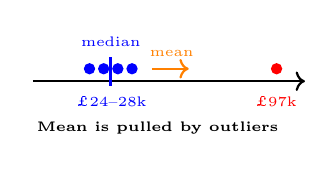
\begin{tikzpicture}[scale=0.72]
  \draw[thick,->] (-0.2,0) -- (4.6,0);
  \foreach \xd in {0.8, 1.05, 1.3, 1.55}{
    \fill[blue] (\xd,0.22) circle (0.1);
  }
  \fill[red] (4.1,0.22) circle (0.1);
  \node[below,font=\tiny,blue] at (1.2,{-0.1})  {£24--28k};
  \node[below,font=\tiny,red]  at (4.1,{-0.1})  {£97k};
  \draw[blue,very thick] (1.175,0.42) -- (1.175,-0.08);
  \node[above,blue,font=\tiny] at (1.175,0.44) {median};
  \draw[->,thick,orange] (1.9,0.22) -- (2.55,0.22);
  \node[above,orange,font=\tiny] at (2.25,0.26) {mean};
  \node[below,font=\tiny\bfseries] at (2.0,{-0.55})
    {Mean is pulled by outliers};
\end{tikzpicture}

\vspace{0.5em}


\end{center}

\column{0.67\textwidth}
\footnotesize
\vspace{0.3em}
\begin{enumerate}\itemsep1pt
  \begin{multicols}{2}
    \item $-6+(-2) = \ashowq{-8}$
    \item $\frac{1}{3}+\frac{1}{2} = \ashowq{\frac{5}{6}}$
  \end{multicols}
  \vspace{-1em}
  \item Median of: $3,\ 9,\ 4,\ 7,\ 1$ \ashow{4}
  \item Mean \textbf{and} median of: $5,\ 8,\ 3,\ 12,\ 7$. Which is larger? \ashow{equal (both $7$)}
  \item Five salaries are: £24k, £26k, £25k, £28k, \textcolor{red}{£97k}. Would you prefer to use the mean or the median to find the average? \ashow{the median}
  \item For $-10,-1,0,2,3$: \textit{estimate} whether the mean is positive or negative. Then calculate both mean and median. \ashow{negative: mean $-1.2$; median $0$}
  \item Find the mean and median of: $-6,\ -2,\ 4,\ -3,\ 7,\ 0$ \ashow{mean $0$; median $-1$}
  \item What is the median of: $\frac{1}{3},\ \frac{3}{4},\ \frac{1}{2},\ \frac{1}{6},\ \frac{2}{3},\ \frac{1}{4}$ \ashow{$\frac{5}{12}$}
  \item True or False?\\
    (a) The median is always one of the values in the dataset. \ashow{False}\\
    (b) The mean and median are always different. \ashow{False}\\
    (c) A very large outlier affects the median more than the mean. \ashow{False}

\end{enumerate}

\end{columns}
\end{frame}

\begin{frame}{Worked Solution: Starter 5, Question 1}
\hypertarget{work-st5}{}
\textbf{Question:} \(-6 + (-2) = ?\)

\textbf{Worked Solution:}
Adding \(-2\) is the same as subtracting \(2\):
\[
-6 + (-2) = -6 - 2 = -8.
\]
\end{frame}

\begin{frame}{Worked Solution: Starter 5, Question 2}
\textbf{Question:} \(\frac{1}{3} + \frac{1}{2} = ?\)

\textbf{Worked Solution:}
Use a common denominator of \(6\):
\[
\frac{1}{3} = \frac{2}{6}
\quad\text{and}\quad
\frac{1}{2} = \frac{3}{6}.
\]
So
\[
\frac{1}{3} + \frac{1}{2}
= \frac{2}{6} + \frac{3}{6}
= \frac{5}{6}.
\]
\end{frame}

\begin{frame}{Worked Solution: Starter 5, Question 3}
\textbf{Question:} Median of \(3, 9, 4, 7, 1\)?

\textbf{Worked Solution:}
Write in order:
\[
1,\ 3,\ 4,\ 7,\ 9.
\]
There are 5 numbers, so the median is the middle value:
\[
4.
\]
\end{frame}

\begin{frame}{Worked Solution: Starter 5, Question 4}
\textbf{Question:} Mean and median of \(5, 8, 3, 12, 7\). Which is larger?

\textbf{Worked Solution:}
In order:
\[
3,\ 5,\ 7,\ 8,\ 12.
\]
So the median is \(7\).

The mean is
\[
\frac{5 + 8 + 3 + 12 + 7}{5}
= \frac{35}{5}
= 7.
\]
They are equal: neither is larger.
\end{frame}

\begin{frame}{Worked Solution: Starter 5, Question 5}
\textbf{Question:} Five salaries are £24k, £26k, £25k, £28k, £97k. Would you prefer to use the mean or the median to find the average?

\textbf{Worked Solution:}
Sort the salaries:
\[
24,\ 25,\ 26,\ 28,\ 97
\]
(in thousands of pounds).

The median is \(26\)k.

The mean is pulled up by the large outlier:
\[
\frac{24 + 25 + 26 + 28 + 97}{5}
= \frac{200}{5}
= 40\text{k}.
\]
The median is more representative, so we should prefer the median.
\end{frame}

\begin{frame}{Worked Solution: Starter 5, Question 6}
\textbf{Question:} For \(-10, -1, 0, 2, 3\): estimate whether the mean is positive or negative. Then calculate both mean and median.

\textbf{Worked Solution:}
The negative numbers dominate: \(-10\) and \(-1\) together are \(-11\), while the positive numbers add to \(5\). So the mean should be negative.

Mean:
\[
\frac{-10 - 1 + 0 + 2 + 3}{5}
= \frac{-6}{5}
= -1.2.
\]

In order:
\[
-10,\ -1,\ 0,\ 2,\ 3.
\]
The median is the middle value:
\[
0.
\]
\end{frame}

\begin{frame}{Worked Solution: Starter 5, Question 7}
\textbf{Question:} Find the mean and median of \(-6, -2, 4, -3, 7, 0\).

\textbf{Worked Solution:}
Mean:
\[
\frac{-6 - 2 + 4 - 3 + 7 + 0}{6}
= \frac{0}{6}
= 0.
\]

In order:
\[
-6,\ -3,\ -2,\ 0,\ 4,\ 7.
\]
There are 6 numbers, so the median is the mean of the two middle values:
\[
\frac{-2 + 0}{2} = -1.
\]
\end{frame}

\begin{frame}{Worked Solution: Starter 5, Question 8}
\textbf{Question:} What is the median of \(\frac{1}{3}, \frac{3}{4}, \frac{1}{2}, \frac{1}{6}, \frac{2}{3}, \frac{1}{4}\)?

\textbf{Worked Solution:}
Write each fraction in twelfths:
\[
\frac{1}{6}=\frac{2}{12},\quad
\frac{1}{4}=\frac{3}{12},\quad
\frac{1}{3}=\frac{4}{12},\quad
\frac{1}{2}=\frac{6}{12},\quad
\frac{2}{3}=\frac{8}{12},\quad
\frac{3}{4}=\frac{9}{12}.
\]
In order:
\[
\frac{2}{12},\ \frac{3}{12},\ \frac{4}{12},\ \frac{6}{12},\ \frac{8}{12},\ \frac{9}{12}.
\]
There are 6 numbers, so the median is halfway between the 3rd and 4th:
\[
\frac{\frac{4}{12} + \frac{6}{12}}{2}
= \frac{10}{12} \div 2
= \frac{5}{12}.
\]
\end{frame}

\begin{frame}{Worked Solution: Starter 5, Question 9}
\textbf{Question:} True or False?
(a) The median is always one of the values in the dataset.
(b) The mean and median are always different.
(c) A very large outlier affects the median more than the mean.

\textbf{Worked Solution:}

(a) \textbf{False.}
For example, in \(1, 2, 3, 4\), the median is
\[
\frac{2 + 3}{2} = 2.5,
\]
which is not in the dataset.

(b) \textbf{False.}
For example, in \(5, 8, 3, 12, 7\), both the mean and median are \(7\).

(c) \textbf{False.}
A very large outlier affects the mean more than the median. The median is resistant to outliers.
\end{frame}

\end{document}